\cchapter{Computations} \label{Chapter:computations}

Apart from visualization, \TexMol also allows users to compute
functions of the molecule including surfaces and surface functions
like isosurfaces, curvatures, and the contour spectrum and volume
functions like electron density and hydrophobicity.

\csection{Isosurfaces}

Given a volume \mm{f(x,y,z)}, an isosurface with isovalue \mm{c} is
defined as \mm{f(x,y,z)=c}. The extraction of isosurfaces from
volume files is known as isocontouring. There are two packages for
isocontouring within \TexMol. One is the \emph{marching cubes}
algorithm implemented in the \emph{Contouring} library and the other
is the \emph{seed set} algorithm implemented in the
\emph{contourlib} library. To create an isosurface, the user needs
to load in a volume and extract it at a given isovalue as described
in table \ref{Table:Isosurfacing}.

\warning{Isosurfacing of large volume files could take up to a
minute.}

\steps{Isosurfacing}{Table:Isosurfacing}{\item Load a volume if it
is not already done and select it in the molecule browser to bring
up its property widget.
\item In the color table, right click at any point and add an
isocontour.
\item This could take a few seconds to a minute or so. \item The
isovalue can be modified by dragging the isosurface bar in the color
table. \item The isosurface can be deleted by deleting its
isosurface bar.}

\subsection{Rendering isosurfaces}

Isosurfaces are rendered by default on creation and cannot be
hidden. We also currently use smooth shading for rendering the
meshes. The color of the mesh at any vertex is given by the color of
the volume at that point. The color of the entire mesh can be
changed by right clicking on the isocontour bar and selecting edit.



\csection{Curvatures}

Using a functional definition for the electron density
representation of a molecule, the curvatures at any point can be
estimated. Analytical definitions of the functions yield analytical
equations for deriving the curvatures. \TexMol estimates two
curvatures, the Mean curvature \mm{H} and the Gaussian curvature
\mm{K}. If \mm{k_{min}} and \mm{k_{max}} are the minimum and maximum
curvatures at a point, then
\begin{equation}
H=\frac{1}{2}( k_{min} + k_{max} ),\; K=k_{min}\times k_{max}
\end{equation}
These are calculated from a potential function \mm{\phi} as follows
\begin{equation}
H=\frac{ C(f_x^2(f_{yy}+f_{zz})) - 2C(f_xf_yf_{xy})
}{2({Cf_x^2}^2)}, \;
K=\frac{2C(f_xf_y(f_{xz}f_{yz}-f_{xy}f_{zz}))}{(C(f_x^2))^2}
\end{equation}

\mm{C} denotes cyclic summation over \mm{x,y,z},\\
subscripts denote partial differentiation with respect to those
variables.

There are two ways in which most functions can be calculated in
\TexMol. First, the user can do it through the graphical user
interface. Second, it can be done in batch mode. In table
\ref{Table:CurvatureEstimation}, we describe how to calculate the
mean and gaussian curvatures from the graphical user interface.

\begin{figure}
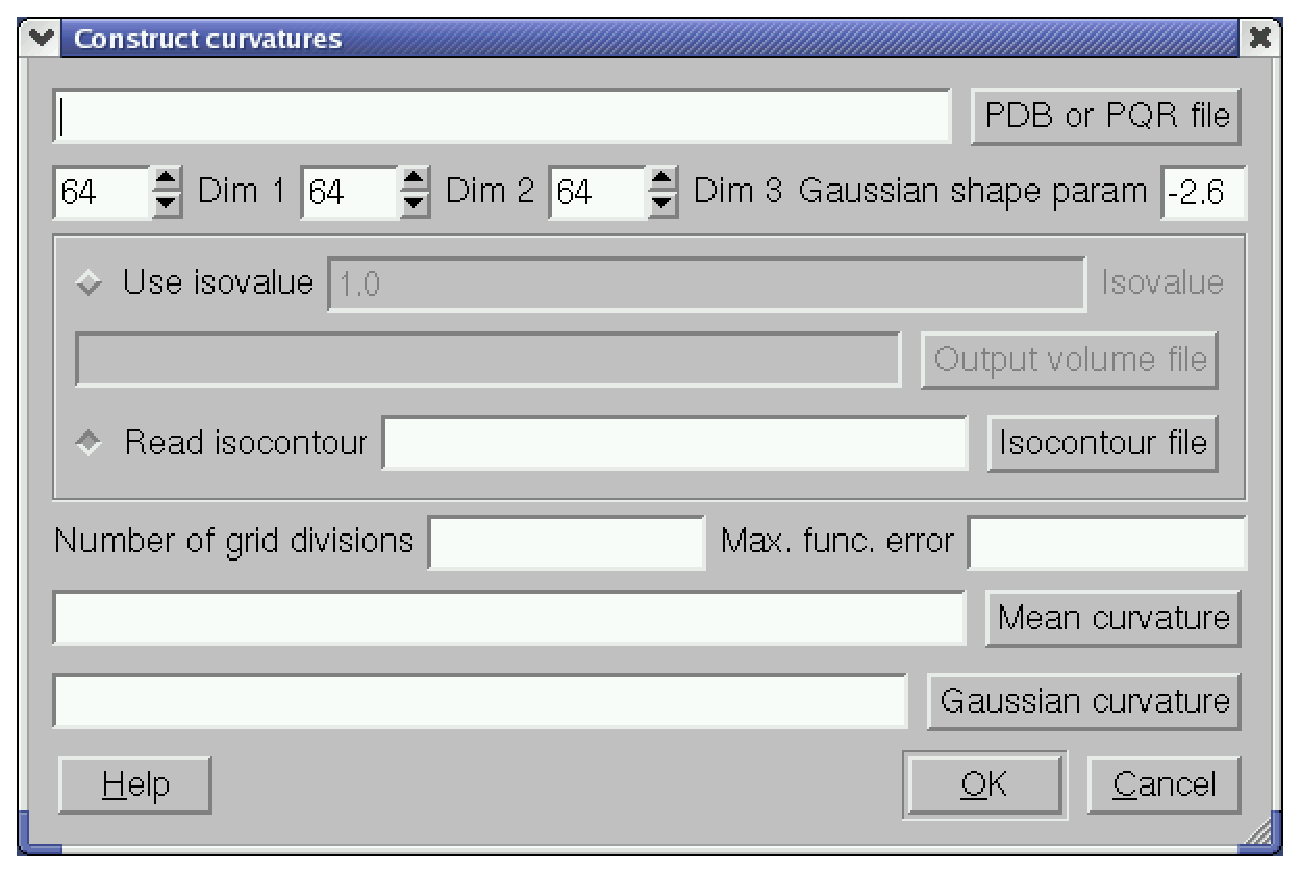
\includegraphics[width=5in]{Images/curvatureWidget.ps}
\ccaption{This curvature widget can be opened by selecting Utilities
- Construct curvatures from the main menu bar.}
\label{Figure:CurvatureEstimation}
\end{figure}

\steps{Estimation of curvatures from
GUI}{Table:CurvatureEstimation}{\item Consider figure
\ref{Figure:CurvatureEstimation} for this example.
\item Load a molecular file to estimate curvatures for. \item Since
we need an electron density function definition, select values for
the volume dimensions and the gaussian blobbyness parameter. \item
If you know the points at which to estimate the curvature, you can
load the mesh file, or ask \TexMol to perform isocontouring at some
selected isovalue. \item The number of grid divisions and the
function error allowed are tradeoffs to performance. \item Three
files, the mean and gaussian curvature, and the curvature values
themselves are written out to the selected files.}

\csection{Electron density}

The electron density has been used as a description of molecular
shape. One commonly used model of sum of radial functions has been
used in \TexMol. This field can be described at any point \mm{x,y,z}
in a volume as a scalar value given by
\begin{equation}
\phi_{dens} = \sum_{i=1}^{M}e^{{\beta}_i} \label{electrondensity}
\end{equation}
and
\begin{equation}
{\beta}_i=blobby*\frac{{(x-xc_i)}^2 + {(y-yc_i)}^2 +
{(z-zc_i)}^2}{{vr_i}^2}-blobby
\end{equation}

\begin{tabular}{ll}
\mm{M} &   is the total number of atoms,\\
\mm{xc_i, yc_i, zc_i} &    is the center of the \mm{i^{th}} atom,\\
\mm{vr_i} &    is the van der Waal radius of atom \mm{i} and \\
\mm{blobby} &  is a parameter which controls the shape of the
gaussian.
\end{tabular}

Using the graphical user interface, the users can compute the
electron density of a molecule as shown in table
\ref{Table:ComputeElectronDensity}.  See \cite{bajaj06fast} for a
fast summation algorithm. There are four types of electron density
volumes we compute with respect to visualization.
\begin{enumerate}
\item Scalar valued electron density.
\item Vector valued electron density, where there are 4 tuples at
each point. RGB at a point contains a color value, and A contains
the density itself. This can be computed in three ways. See figure
\ref{Figure:RawVVOlumes} for an example.
    \begin{enumerate}
    \item Color according to a structure like atoms, residues etc.
    \item Color using the specifications in a color map file.
    \item Use depth coloring to bring out surface features. This
    feature currently takes as input a volume file ( scalar or
    volume ). Load a volume file and select Utilities, Construct
    depth colored volume from the menu bar.
    \end{enumerate}
\end{enumerate}

\begin{figure}
     \centering
     \subfigure[Volume with colors assigned to secondary structures, blurred at the atomic level]{
          \label{Figure:RawVVOlumesa}
          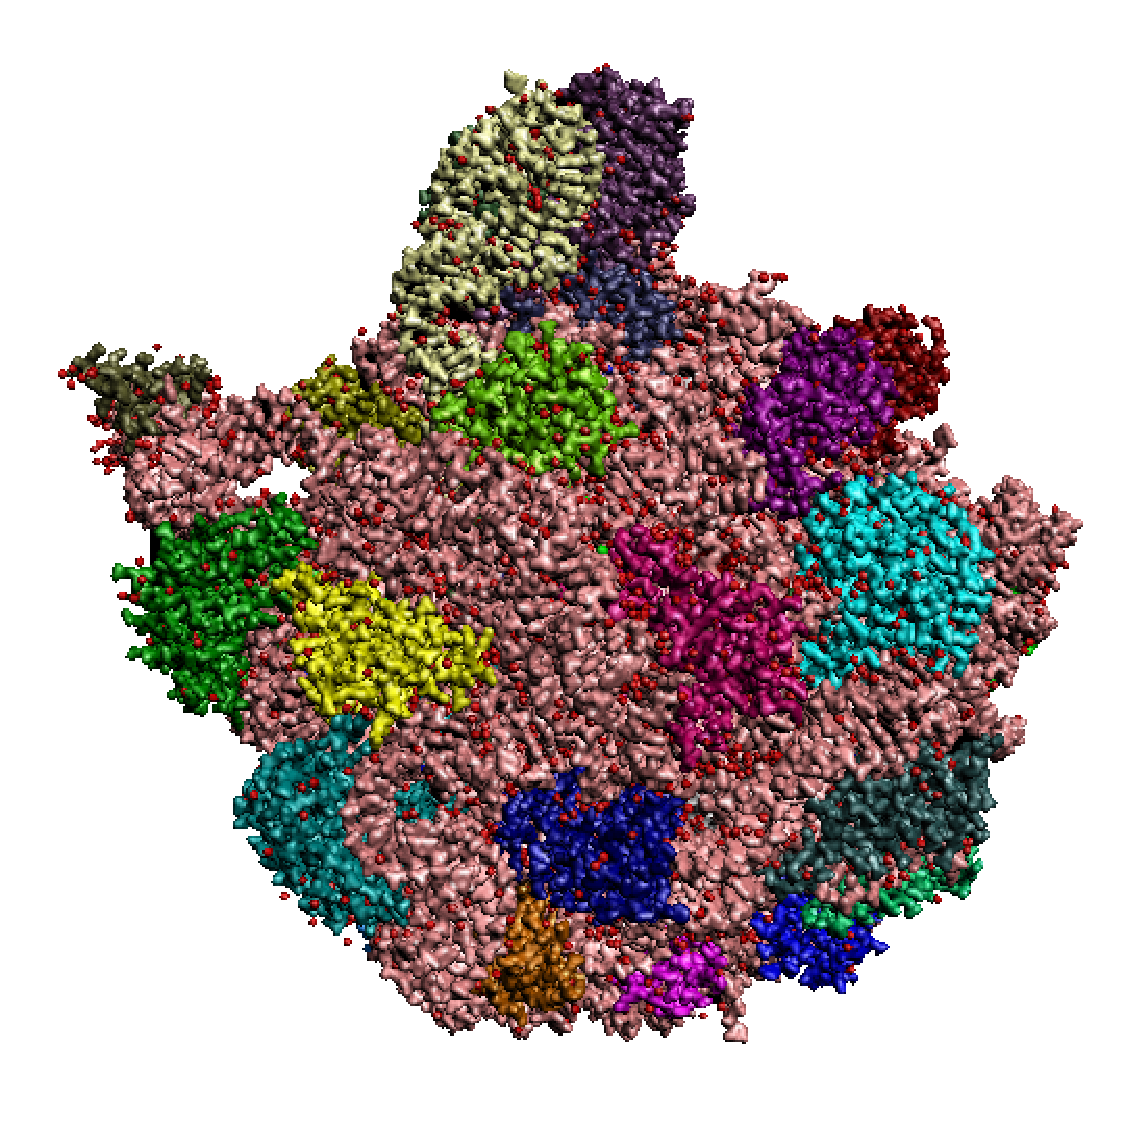
\includegraphics[width=.45\textwidth]{Images/Ribosome_volume_high_res.ps}}
     \hspace{.3in}
     \subfigure[Volume with colors assigned to secondary structures, blurred at the residue level]{
          \label{Figure:RawVVOlumesb}
          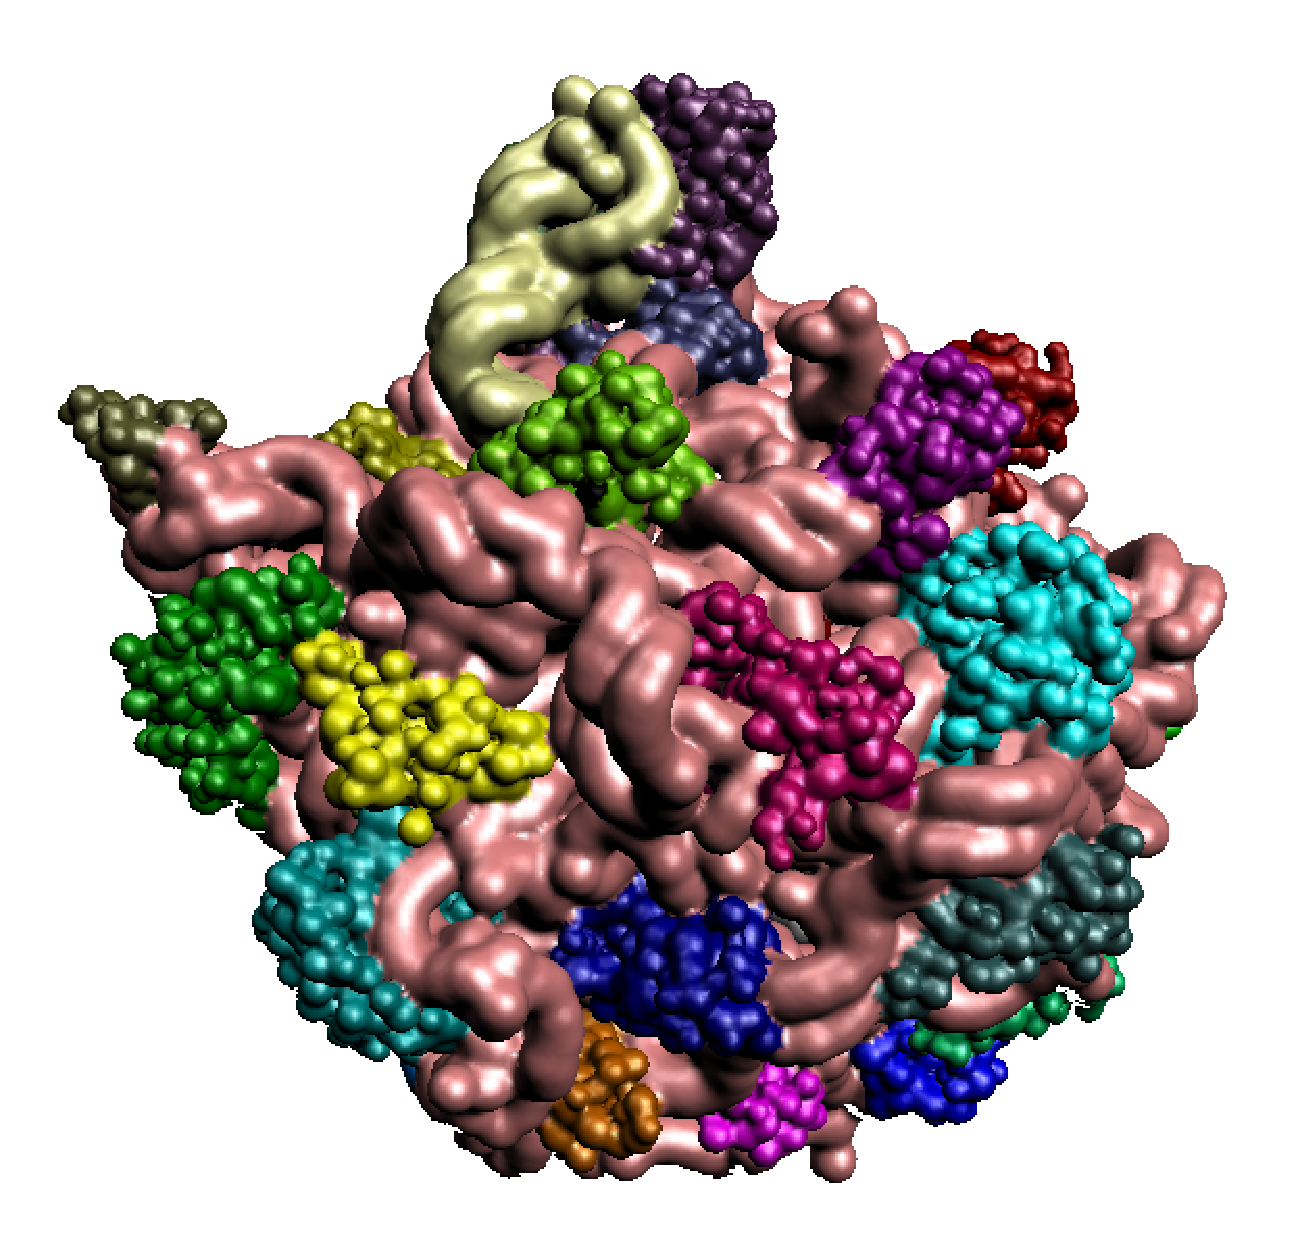
\includegraphics[width=.45\textwidth]{Images/Ribosome_volume.ps}}\\
     \vspace{.3in}
     \subfigure[In order to show specific atoms like the iron in the heme structure of the hemoglobin, we can use a color map file.]{
          \label{Figure:RawVVOlumesc}
          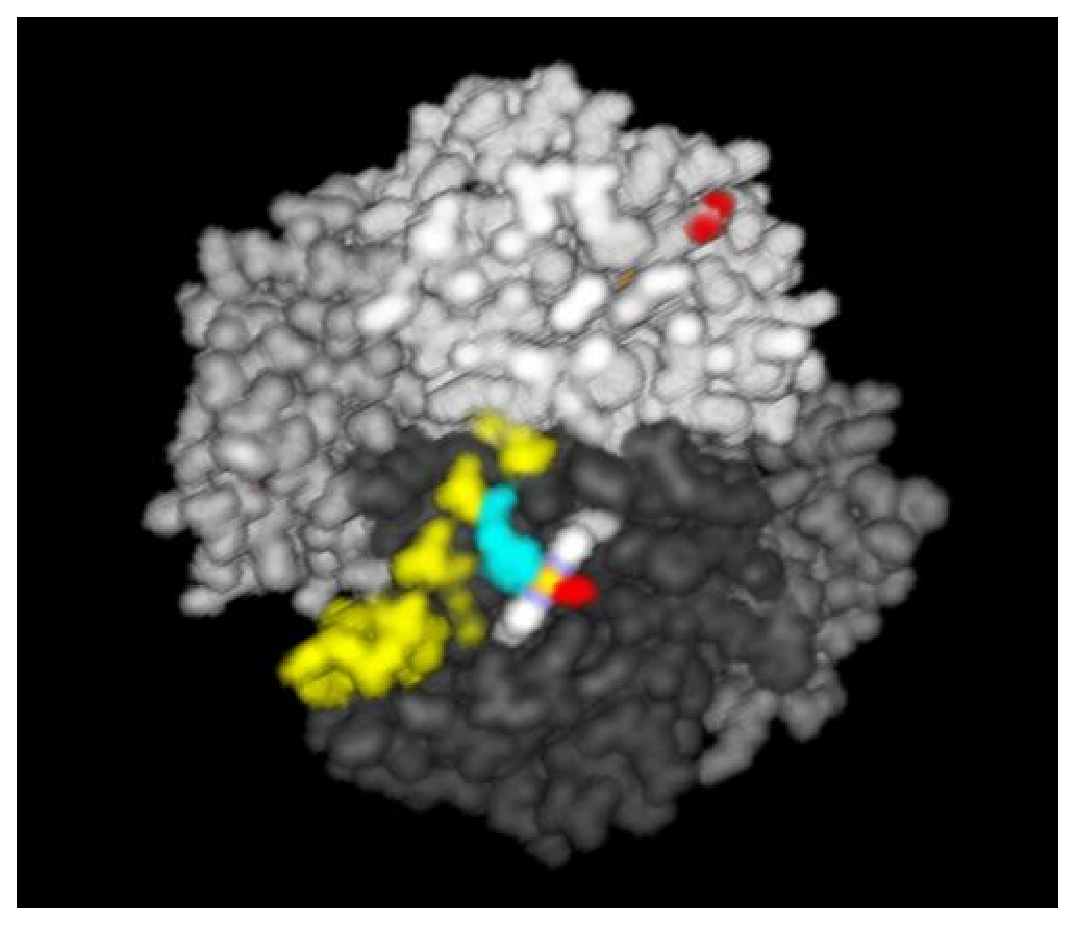
\includegraphics[width=.45\textwidth]{Images/heme.ps}}
     \hspace{.3in}
     \subfigure[A virus (1lp3.pdb) rendered as an isosurface of a depth colored volume showing its surface features]{
          \label{Figure:RawVVOlumesd}
          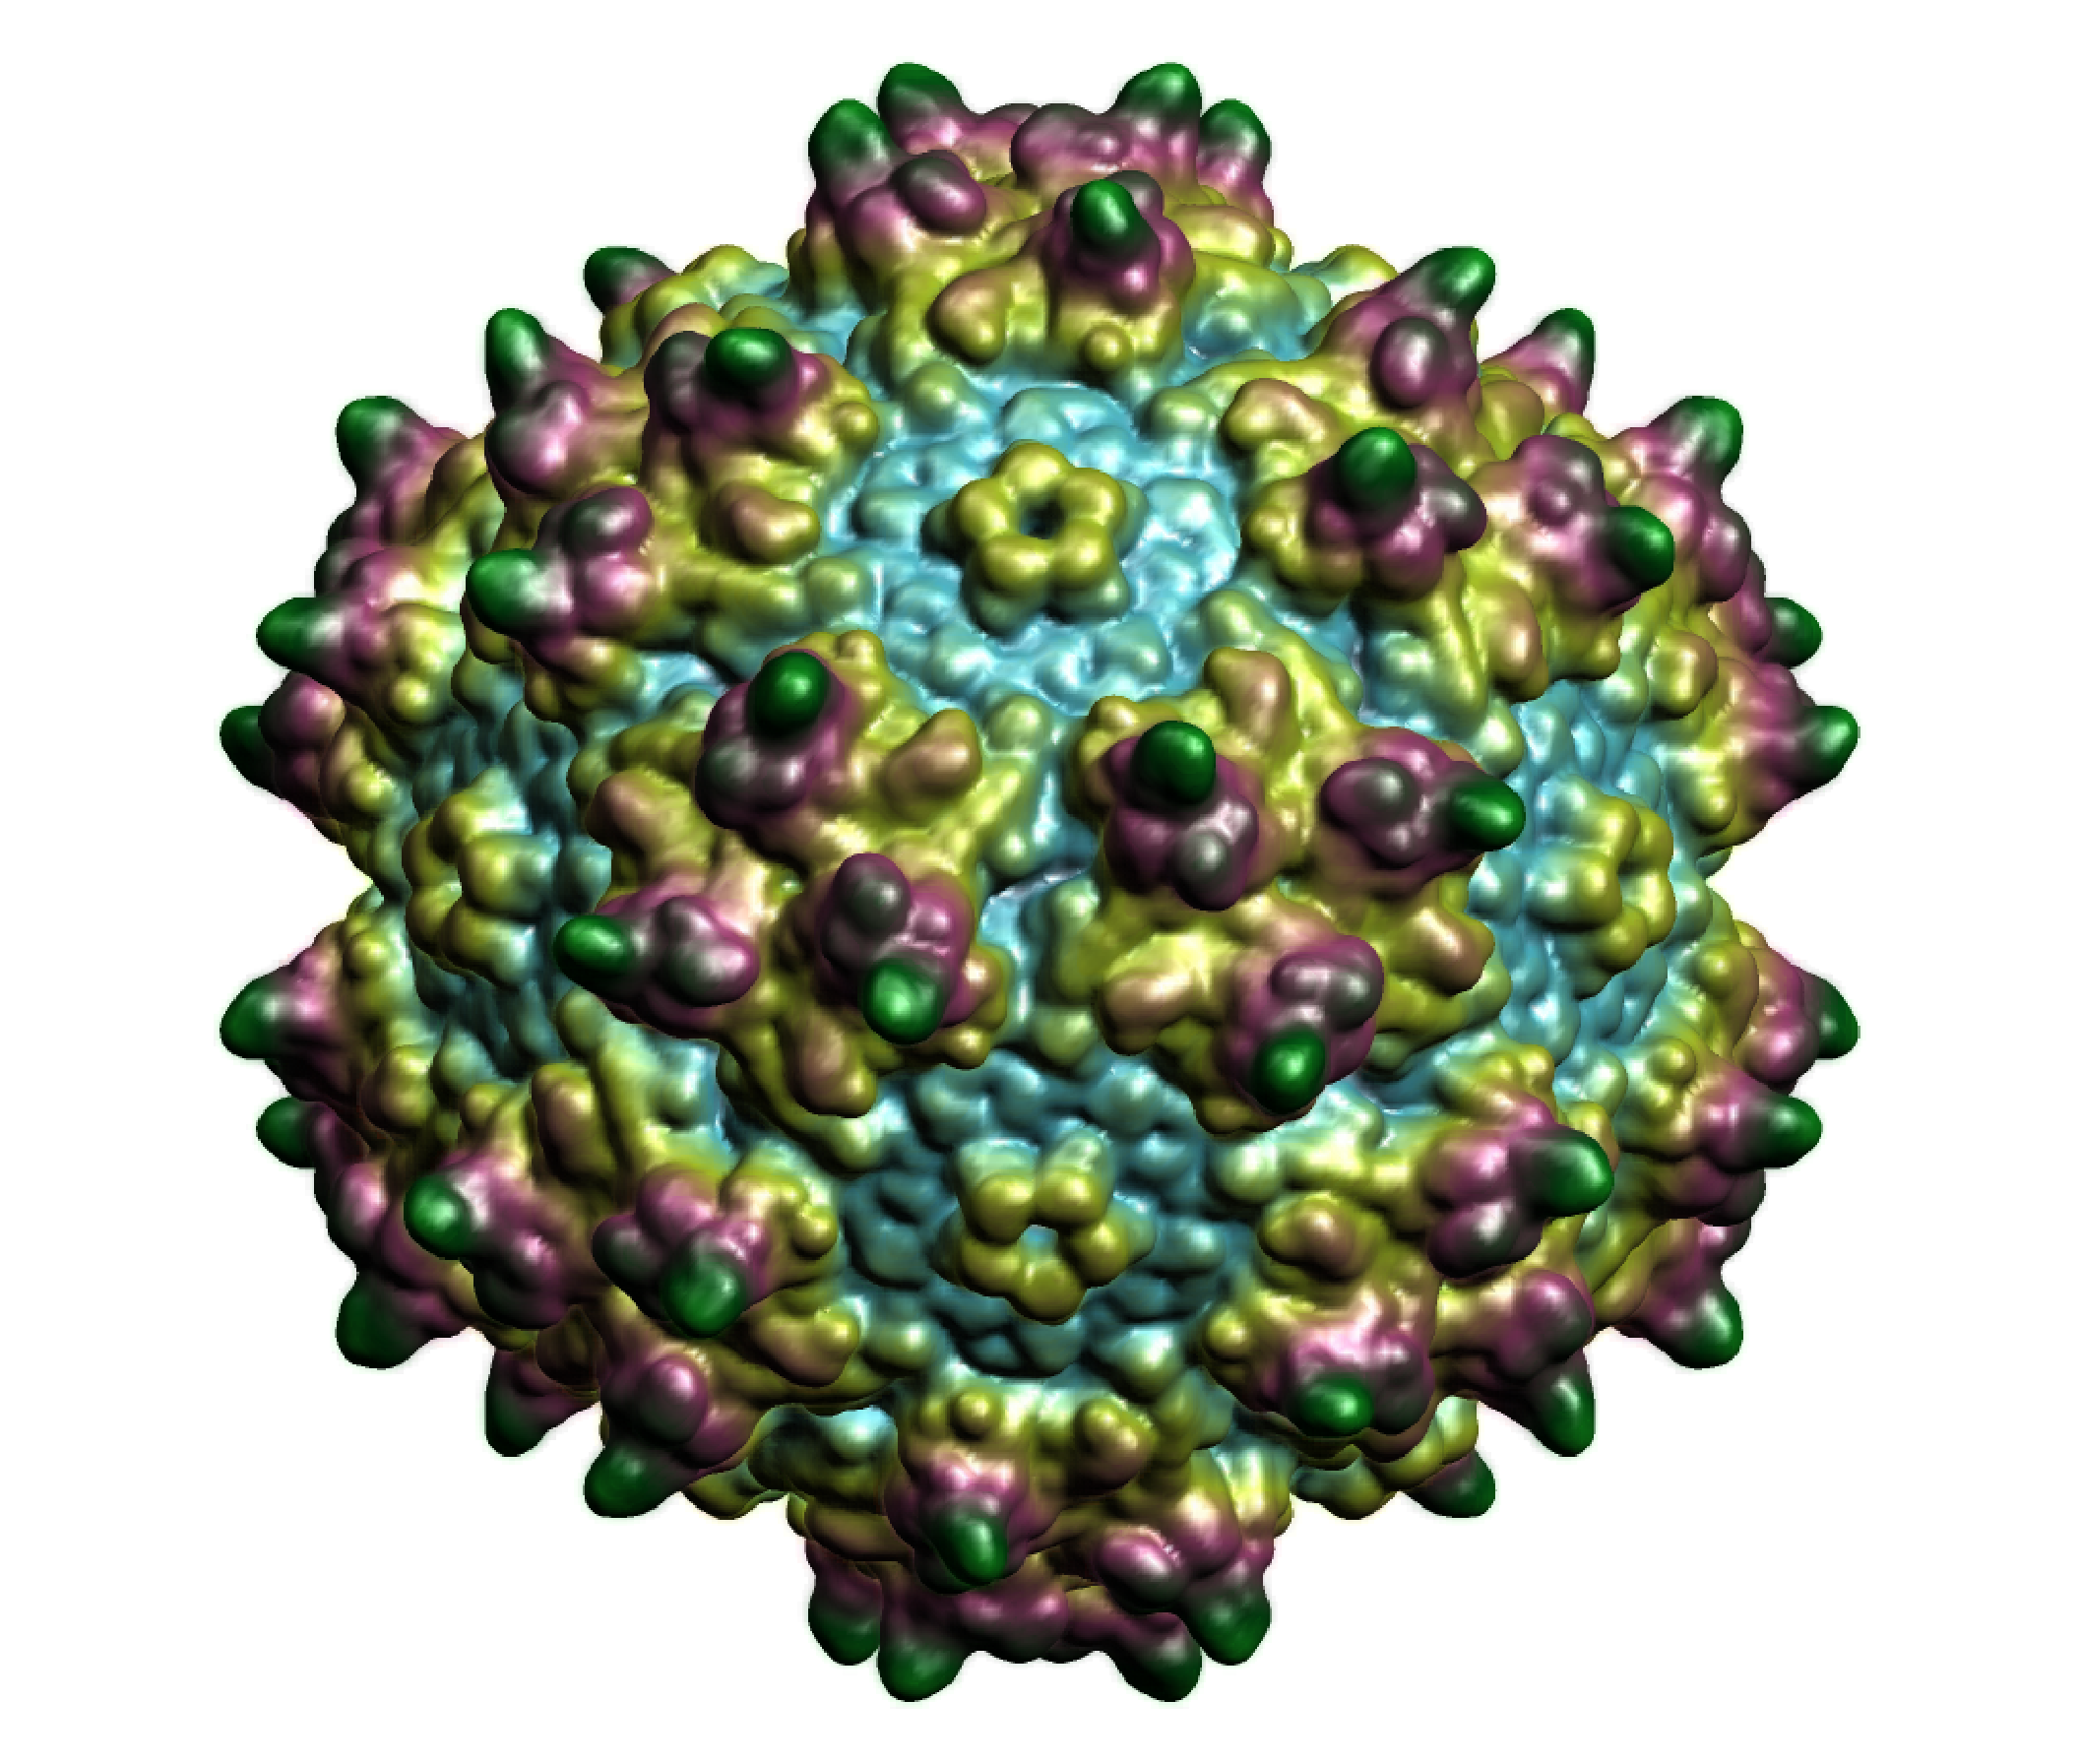
\includegraphics[width=.45\textwidth]{Images/1lp3.ps}}\\
     \caption{Vector valued volumes constructed in different ways to bring out different features.}
     \label{Figure:RawVVOlumes}
\end{figure}


\steps{Electron density
computation}{Table:ComputeElectronDensity}{\item Load a molecule
file if it is not already loaded. \item Select the molecule from the
molecule browser. \item Select Utilities and Construct volume from
the menu bar. \item Select Electron density as the function needed
to be computed and give the dimensions and blobbyness parameter.
\item If you need a output file, then enter a output file name, or
just leave it blank.
\item RawV volumes or vector valued volumes can also be constructed by
choosing it in the check box. \item If rawV was chosen, then also
choose a color LOD for the density. \item The generated volume can
be loaded in to memory or not by checking Load generated volume. }

\csection{Hydrophobicity}

Hydrophobicity maps can be created in a similar fashion as rawiv
electron density files. Follow the procedure outlined in table
\ref{Table:ComputeElectronDensity}, but choose hydrophobicity
instead of electron density. You probably cannot create anything
meaningful by choosing hydrophobicity and color mapped volumes
together. The hydrophobicity is given per atom as shown in the table
in file \emph{elementInformation.h}. The hydrophobicity of the
dengue virus capsid protein (1r6r.pdb) is shown in figure
\ref{Figure:Hydrophobicity}.

\begin{figure}
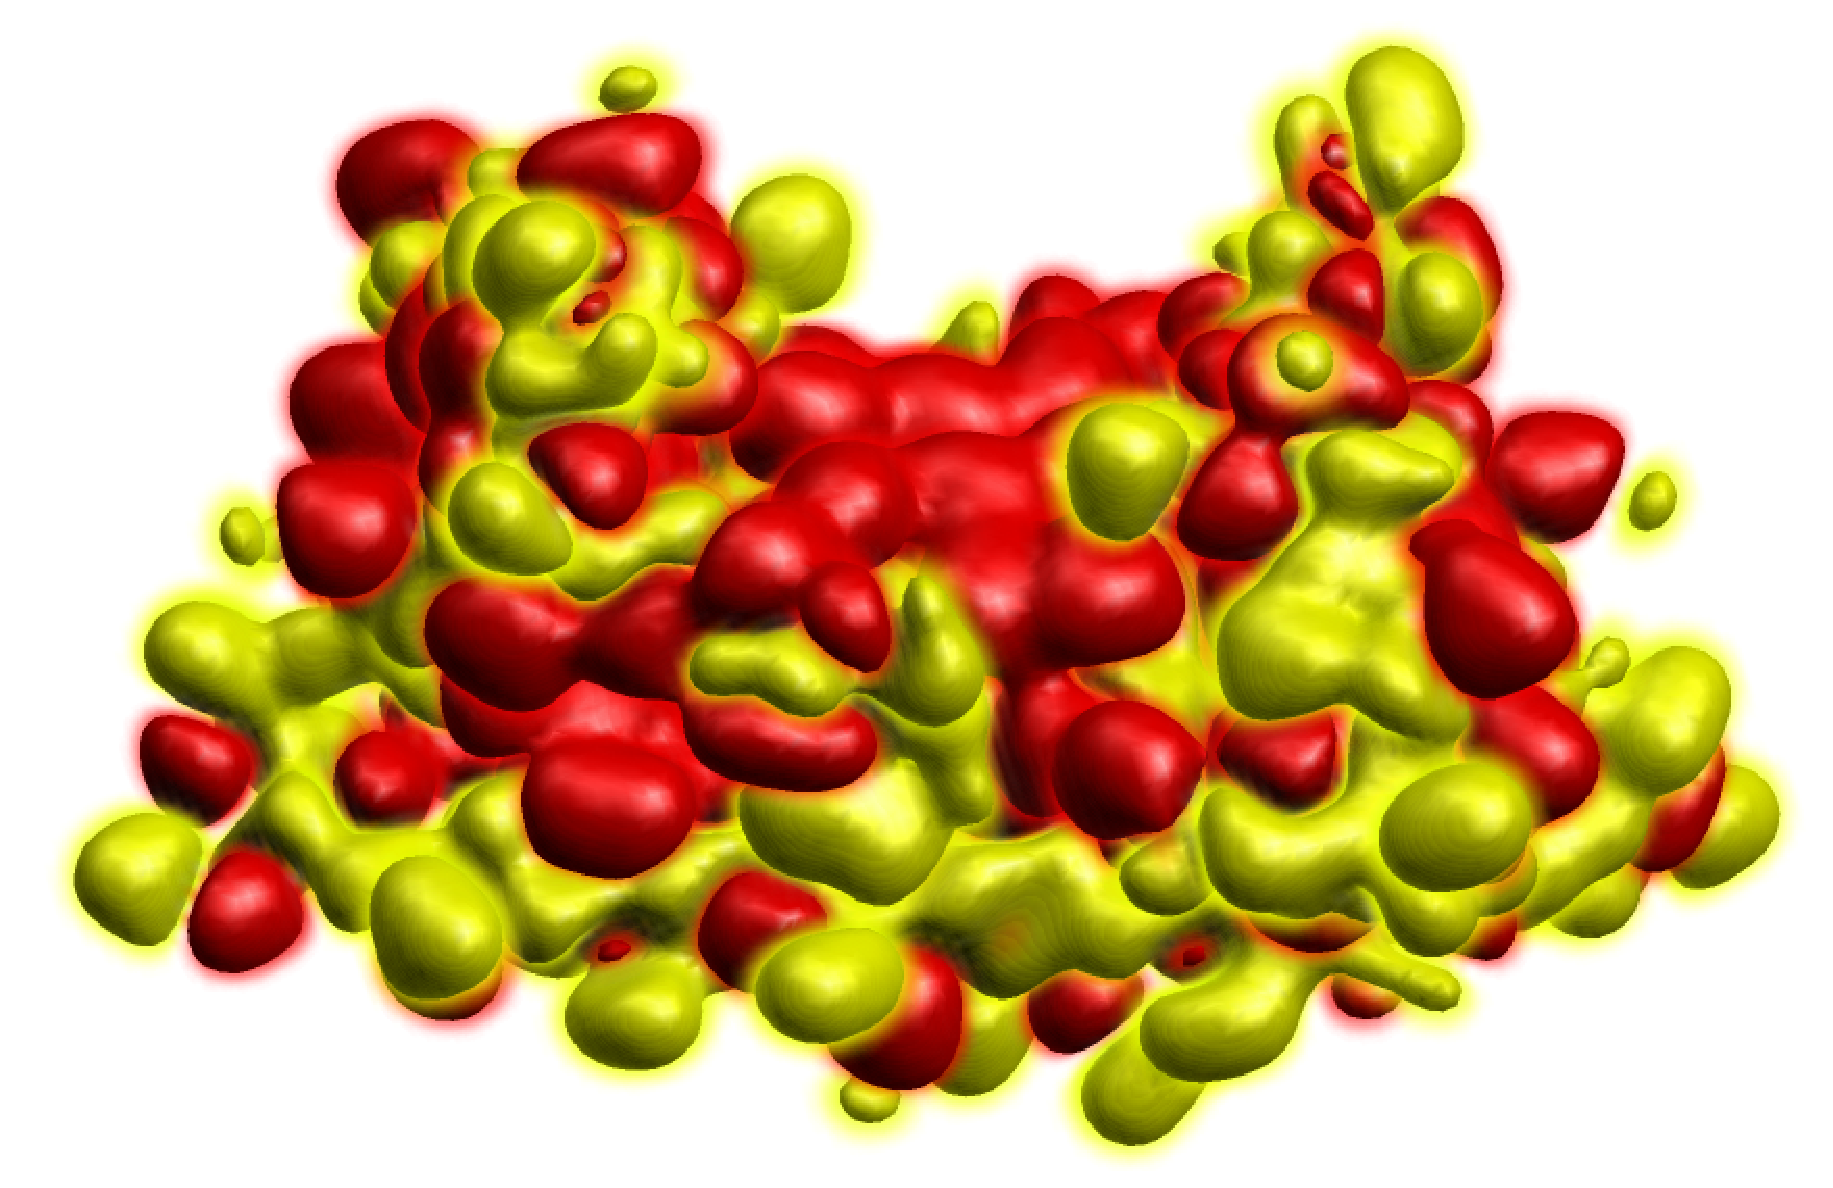
\includegraphics[width=5in]{Images/1r6r_hydro4.ps}
\ccaption{Hydrophobicity volume rendering of the dengue virus capsid
protein (1r6r.pdb). The hydrophobic regions are in yellow and the
hydrophillic regions are in red.} \label{Figure:Hydrophobicity}
\end{figure}


\csection{Contour spectrum}

The contour spectrum is used for obtaining quantitative information
about the volume files. The documentation for the contour spectrum
can be found in the user manual for CCV's volume rover.
